%% LyX 2.3.2 created this file.  For more info, see http://www.lyx.org/.
%% Do not edit unless you really know what you are doing.
\documentclass[11pt,twoside,british,t]{beamer}
\usepackage{amstext}
\usepackage{amssymb}
\usepackage{fontspec}
\usepackage{unicode-math}
\setmainfont[Mapping=tex-text]{TeX Gyre Schola}
\setsansfont[Scale=0.91,Mapping=tex-text]{Segoe UI}
\setmonofont[Scale=0.95]{Consolas}
\setcounter{secnumdepth}{3}
\setcounter{tocdepth}{3}
\setlength{\parskip}{\medskipamount}
\setlength{\parindent}{0pt}
\usepackage{endnotes}

\makeatletter

%%%%%%%%%%%%%%%%%%%%%%%%%%%%%% LyX specific LaTeX commands.
\pdfpageheight\paperheight
\pdfpagewidth\paperwidth


%%%%%%%%%%%%%%%%%%%%%%%%%%%%%% Textclass specific LaTeX commands.
% this default might be overridden by plain title style
\newcommand\makebeamertitle{\frame{\maketitle}}%
% (ERT) argument for the TOC
\AtBeginDocument{%
  \let\origtableofcontents=\tableofcontents
  \def\tableofcontents{\@ifnextchar[{\origtableofcontents}{\gobbletableofcontents}}
  \def\gobbletableofcontents#1{\origtableofcontents}
}
\let\footnote=\endnote

\@ifundefined{date}{}{\date{}}
%%%%%%%%%%%%%%%%%%%%%%%%%%%%%% User specified LaTeX commands.
\usepackage{xcolor}
\usepackage{xpatch}

\definecolor{AccentB80}{RGB}{197, 213, 255}
\definecolor{AccentB60}{RGB}{139, 171, 255}
\definecolor{AccentB40}{RGB}{81,  130, 255}
\definecolor{Accent}   {RGB}{0,   63,  221}
\definecolor{AccentD25}{RGB}{0,   46,  165}
\definecolor{AccentD50}{RGB}{0,   31,  110}

\setlength{\parskip}{0pt}
\newcommand{\zwnbsp}{}

\definecolor{blue}{HTML}{0000F0} % 
\definecolor{purple}{HTML}{700090}
\definecolor{orange}{HTML}{F07000}
\definecolor{teal}{HTML}{0090B0}
\definecolor{brown}{HTML}{A00000}
\definecolor{green}{HTML}{008000}
\definecolor{pink}{HTML}{F000F0}
\usecolortheme[named=pink]{structure}

\newcommand{\pars}{\medskip}
\newcommand{\parj}{\vspace{-\medskipamount}}

\setbeamercolor{title}{fg=Accent}
\setbeamercolor{example text}{fg=AccentB40}
\setbeamerfont{title}{size=\Huge}

\setbeamercolor{local structure}{fg=black}
\setbeamerfont{local structure}{size=\normalsize}
\setbeamertemplate{itemize item}{•}
\setbeamertemplate{itemize subitem}{◦}

\setlength{\labelsep}{0.63cm}
\setlength{\topsep}{0cm}
\setlength{\leftmargini}{0.63cm}
\setlength{\leftmarginii}{\leftmargini}
\newcommand{\linebox}[1]{%
	\parbox{\textwidth}{\rule{0cm}{1em}\strut\smash{#1}\strut}}

\xpatchcmd{\itemize}{\def\makelabel}{% Configure inside itemize
	\setlength{\topsep}{0pt}%
	\setlength{\itemsep}{0pt}%
	\def\makelabel}{}{}
\xpatchcmd{\itemize}{\llap}{\rlap}{}{}
\xpatchcmd{\beamer@enum@}{\llap}{\rlap}{}{}
\setbeamertemplate{itemize/enumerate body begin}{}
\setbeamertemplate{itemize/enumerate body end}{\pars}

\setbeamertemplate{itemize/enumerate subbody begin}{\pars}
\setbeamerfont{itemize/enumerate body}{size=\parj}
\setbeamerfont{itemize/enumerate subbody}{size=\parj}
	
\setbeamercolor{author}{fg=AccentB40}
\setbeamerfont{author}{size=\large}
\setbeamerfont{institute}{size=\normalsize}

\newsavebox{\mybox}
\newlength{\myboxwidth}

\newcommand{\thefooter}{}
\setbeamertemplate{footline}{%\printinunitsof{cm}\prntlen{}%
	\vspace{-0.13cm}%
	\parbox[b][1cm][t]{\textwidth}{\thefooter}\vspace{1cm}%
}
\renewcommand{\makebeamertitle}{%
	{%
\renewcommand{\thefooter}{%
		\centering \normalsize	\textsuperscript{1}\email{isaac@ecs.vuw.ac.nz} \textsuperscript{2}\email{marco.servetto@ecs.vuw.ac.nz} }%
		\begin{frame}%
		\maketitle%
		\end{frame}%
	}
}%


\setbeamertemplate{block example begin}{%
	\setlength{\fboxsep}{0pt}
	\par\pars%
	\savebox{\mybox}{\usebeamercolor{block title example}\colorbox{bg}{\color{fg}%
			\rule{0cm}{1em}\insertblocktitle:\hspace{0.5em}\strut}}%
	\setlength{\myboxwidth}{\wd\mybox}%	
	\usebox{\mybox}%
	\begin{beamercolorbox}[wd=\dimexpr\textwidth-\myboxwidth]{block body example}%
		\rule{0cm}{1em}\begin{minipage}[t]{4cm}}
\setbeamertemplate{block example end}{%
		\end{minipage}\strut
	\end{beamercolorbox}}


\setbeamerfont{frametitle}{size=\Large} % 14pt
\setbeamercolor{frametitle}{fg=AccentD50}
\newlength{\parprefix}
\setbeamertemplate{frametitle}{%
	\begin{beamercolorbox}{frametitle}%
		\usebeamerfont{frametitle}%
		{\color{AccentD25} \hrule height 0.75pt \vspace{3pt} \hrule height 1.5pt}%
		\setlength{\fboxsep}{0pt}%
		\colorbox{AccentB60}{\linebox{\ \insertframetitle}}%
		{\color{AccentD25} \hrule height 1.5pt \vspace{3pt} \hrule height 0.75pt}%
		\pars%
		\vspace{\dimexpr-0.41cm}%
	\end{beamercolorbox}}

\usepackage{fontspec} % To set xetex fonts
\setmainfont[Ligatures={Common, Discretionary}, Scale=0.9090909090909091]{TeX Gyre Schola}
\setmonofont[Ligatures={Discretionary}, Scale=0.9545454545454545]{Consolas} % 10.5/11
\setsansfont[Ligatures={Discretionary}, Scale=0.9090909090909091]{Segoe UI} %10/11

\unimathsetup{math-style=ISO}
\setmathfont[Scale=0.9090909090909091]{TeX Gyre Schola Math}

\usepackage{hyperref}

\hypersetup{colorlinks,urlcolor=[RGB]{0, 155, 240}}
\newcommand{\email}[1]{%
	\href{mailto:#1}{\texttt{#1}}
}
\raggedright
\usepackage{soul}
\newcommand{\comment}[1]{\note{\hl{#1}}}
\usefonttheme{professionalfonts}

\newcommand{\heading}[1]{%
	%3       Blue    /12pt   Blue    /1pt    +0.75pt
	{\vspace{5pt}\color{Accent}%
	\linebox{\large #1}%
	\hrule height 1pt}\vspace{5pt}}

\beamertemplatenavigationsymbolsempty

\setbeamersize{text margin left=1cm, text margin right=1cm} % default is 1cm*1cm
\setbeamersize{sidebar width left=0pt, sidebar width right=0pt}
\geometry{papersize={16cm,12cm}, vmargin=1cm}

\usepackage{tikz}
\usepackage{mathtools}
\usetikzlibrary{calc, positioning}
\newlength{\W}
\settoheight{\W}{\ttfamily W}

\makeatother

\usepackage{polyglossia}
\setdefaultlanguage[variant=british]{english}
\begin{document}
\title{Callability Control}
\author{By Isaac Oscar Gariano\textsuperscript{1} and Marco Servetto\textsuperscript{2}}
\institute{(Victoria University of Wellington)}

\makebeamertitle
\global\long\def\empty{\zwnbsp}%

\global\long\def\k#1{\textcolor{blue}{\texttt{#1}}}%
\global\long\def\t#1{\textcolor{teal}{#1}}%
\global\long\def\f#1{\textcolor{purple}{#1}}%
\global\long\def\l#1{\textcolor{brown}{#1}}%
\global\long\def\v#1{\textcolor{orange}{#1}}%
\global\long\def\m#1{\textcolor{green}{#1}}%

\global\long\def\c#1{\texttt{#1}}%
\global\long\def\ck#1{\c{\k{#1}}}%
\global\long\def\ct#1{\c{\t{#1}}}%
\global\long\def\cf#1{\c{\f{#1}}}%
\global\long\def\cv#1{\c{\v{#1}}}%
\global\long\def\cm#1{\c{\m{#1}}}%
\global\long\def\cl#1{\c{\l{#1}}}%

\global\long\def\tab{\texttt{\ \ }}%

\global\long\def\calls#1{\ck{calls[}#1\ck ]}%

\begin{frame}{Conventions}

We will consider C♯ (or other .Net or JVM languages), since it\pars
\begin{itemize}
\item is statically-typed,
\item supports named/identifiable functions (e.g. static/instance methods
and constructors),
\item supports dynamic dispatch (with interfaces, virtual methods, etc.),
\item supports dynamic code loading, and
\item supports dynamic function lookup and invocation (with reflection).
\end{itemize}
\note{It will work on any other statically typed language with named functions,
such as C or Haskell}

For brevity I will omit accessibility modifiers and allow free standing
static functions.
\end{frame}
%
\begin{frame}[<+->]{The Problem}
\begin{enumerate}
\item What \emph{could} this code do?

$\texttt{\ensuremath{\ck{static}} \ensuremath{\ck{void}} \ensuremath{\cf{M1(}\cf )} \{ \ensuremath{\cf{Sign(}\cl 0\cf )}; \}}$

\note{Well it looks like it does nothing, it just gets the sign of 0 (which
is 0) and discards the result. But how do we know Sign won’t send
sensitive information to a third-party?\comment{ I prefered my Russia version… }Well
the documentation dosn’t say it will, and we trust the implementer,
Microsoft, to follow it. But, if we didn’t trust it, what could we
do?}\pars
\item What about this, what \emph{could} it do?

\comment{Note: I am now using a user-defined interface, so that I can freely
play with it’s declaration }

$\texttt{\ensuremath{\ck{interface}} \ensuremath{\ct I} \{ \ensuremath{\ck{void}} \ensuremath{\cf{Run()}}; \}}$\\
$\texttt{\ensuremath{\ck{static}} \ensuremath{\ck{void}} \ensuremath{\cf{M2(}\ct I} \ensuremath{\cv x\cf )} \{ \ensuremath{\cv x}.\ensuremath{\cf{Run()}}; \}}$

\note{This one can do anything the language will let it, so it is likely
to be memory and type safe. However it can still do all sorts of stuff,
like perform I/O or use reflection to inspect and invoke arbitrary
code. The reason why we don’t know what this can do is that I.Run,
is a virtual method, this means that it is dynamically dispatched
and in this case, literally anyone can override it. So we have to
trust the writer of every class that x could be at run-time.}
\item How about this?

$\texttt{\ensuremath{\ck{static}} \ensuremath{\ck{void}} \ensuremath{\cf{M3(}\ct{String}} \ensuremath{\cv{url}\cf )} \{}$\\
$\texttt{\ensuremath{\tab\cm{// Load code (possibly from the internet)}}}$\\
$\texttt{\ensuremath{\tab\ct{Assembly}} \ensuremath{\cv{code}} = \ensuremath{\ct{Assembly}}.\ensuremath{\cf{LoadFrom(}\cv{url}\cf )};}$\\
$\texttt{\ensuremath{\tab\cv{\cv{code}.\cf{GetMethod(}\cl{"M"}\cf )}}.\ensuremath{\cf{Invoke(}\ck{null}}, \ensuremath{\ck{null}\cf )}; \} \ensuremath{\cm{// call \cf{M()}}}}$

\note{This is very problematic, url could refer to code written by anyone,
it might not have even been written yet when M3 was written. So we
cannot inspect the code or simply trust their authors.}
\end{enumerate}
\end{frame}
%
\begin{frame}{Callability}
\begin{itemize}
\item \emph{Callability} is the \emph{ability} to \emph{call} a function.
\item A function’s callability is the set of things it can call.
\end{itemize}
\note{We will abstract away performing an ‘operation’ (such as reading a
file, create a new object, doing integer addition etc) as calling
a named function In this way we can look at a functions callability
to constrain what a function can do. /{*} Improve: For example if
it only has the ability to call functions we know wont read from the
file system, then we know it wont.{*}/}

\pause{\parj}

\heading{Restatement of the Problem: }
\begin{enumerate}
\item What is the callability of $\cf{Sign}$? (Where $\cf{Sign}$ is a
static method.)
\item What is the callability of $\cv x.\cf{Run}$? (Where $\cv x$ is of
an interface type $\ct I$.)
\item What is the callability of $\cf M$? (Where $\cf M$ was a dynamically
loaded static-method.)
\end{enumerate}
\note{We will present a system that can answer these questions by constraining
their callabilities.}
\end{frame}
%
\begin{frame}{The Callability Rules}

\note{As part of type-checking, whenever their is a call to g from within
the body of a function f, we will check that f 'can call' g.}

$\f f\rightsquigarrow\f g$, i.e. a function $\f f$\emph{ can-call}
a function $\f g$, iff:\pars

\pause{}
\begin{enumerate}
\item $\f g\in Calls(\f f)\Rightarrow\f f\rightsquigarrow\f g$,\quad{}i.e.
$\f f$ is annotated with $\calls{\dots,\f g,\dots}$.

\note{A function declaration can be suffixed with a calls annotation with
a list of function names.}
\begin{exampleblock}{Example}

$\texttt{\ensuremath{\ck{static}} \ensuremath{\ck{void}} \ensuremath{\cf{Write(}\ct{String}} \ensuremath{\cv s\cf )} \ensuremath{\calls{\cf{WriteChar}}} \{}$\\
$\texttt{\ensuremath{\tab\ck{foreach (}\ct{Char}} \ensuremath{\cv c} \ensuremath{\ck{in}} \ensuremath{\cv s\ck )} \ensuremath{\cf{WriteChar(}\cv c\cf )}; \}}$\pars
\end{exampleblock}

\pause{}
\item $(\forall\f h\in Calls(\f g)\bullet\f f\rightsquigarrow\f h)\Rightarrow\f f\rightsquigarrow\f g$,\quad{}i.e.
if $\f f$ can call every function in the $\calls{\ldots}$ annotation
of $\f g$.

\note{this makes sense, since you could have just inlined the body of g,
so you're not really gaining any power. Note that if calls(f) is empty,
that this vacously holds}
\begin{exampleblock}{Example}

$\texttt{\ensuremath{\ck{static}} \ensuremath{\ck{void}} \ensuremath{\cf{WriteLine(}\ct{String}} \ensuremath{\cv s\cf )} \ensuremath{\calls{\cf{WriteChar}}} \{}$\\
$\texttt{\ensuremath{\tab\cf{Write(}\v s} \ensuremath{\cf +} \ensuremath{\cl{"\backslash n"}\cf )}; \}}$
\end{exampleblock}
\end{enumerate}

\pause{}

The previous rules apply transitively, and always allow for recursive
calls.\parj
\begin{exampleblock}{Example}

$\texttt{\ensuremath{\ck{static}} \ensuremath{\ck{void}} \ensuremath{\cf{HelloWorld(}\cf )} \ensuremath{\calls{\cf{WriteLine}}} \{}$\\
$\texttt{\ensuremath{\tab\cf{\cf{WriteLine(}}\cl{"Hello World!"}\cf )}; \}}$\\
$\texttt{\ensuremath{\ck{static}} \ensuremath{\ck{void}} \ensuremath{\cf{Main(}\ct{String[]}} \ensuremath{\cv{args}\cf )} \ensuremath{\calls{\cf{WriteChar}}} \{}$\\
$\texttt{\ensuremath{\tab\cf{HelloWorld()}}; \}}$

\pars
\end{exampleblock}
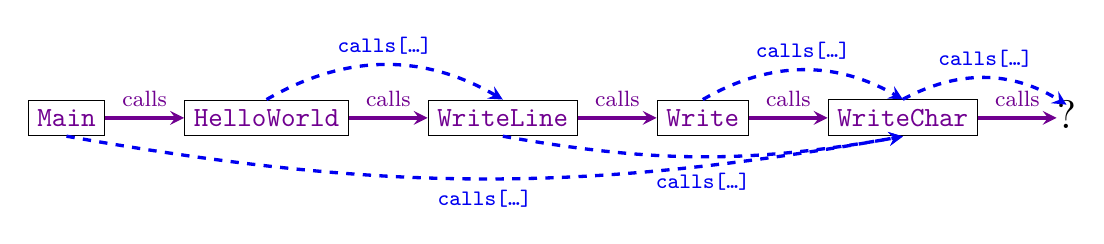
\begin{tikzpicture}[>=stealth]
	\tikzstyle{func} = [draw, font=\ttfamily, text=purple]
	\tikzstyle{call} = [->, color=purple, very thick];
	\tikzstyle{cancall} = [call, color=blue, dashed, very thick];

	\tikzstyle{cancallu} = [cancall, bend left = 30];
	\tikzstyle{cancalld} = [cancall, bend right = 10];

	\tikzstyle{labelt} = [anchor=south, font={\footnotesize{calls}}];
	\tikzstyle{labelc} = [font={\footnotesize{\color{blue} \ttfamily calls[\ldots]}}];
	\tikzstyle{labelu} = [anchor=south, labelc];
	\tikzstyle{labeld} = [anchor=north, labelc];
	
	\node[func, name=M]{Main};
	\node[func, name=HW, right = of M]{HelloWorld};
	\node[func, name=WL, right = of HW]{WriteLine};
	\node[func, name=W, right = of WL]{Write};
	\node[func, name=WC, right = of W]{WriteChar};
	\node[func, name=R, right = of WC, draw=none, text=black]{\begin{minipage}[c][\W]{0cm}\clap{\centering \Large $?$}\end{minipage}};

	\draw (M.east) edge[call] node[labelt]{} (HW.west); 
	\draw (HW.east) edge[call] node[labelt]{} (WL.west); 
	\draw (WL.east) edge[call] node[labelt]{} (W.west); 
	\draw (W.east) edge[call] node[labelt]{} (WC.west); 
	\draw (WC.east) edge[call] node[labelt]{} (R.west); 

	\draw (HW.north) edge[cancallu] node[labelu]{} (WL.north); 
	\draw (W.north) edge[cancallu] node[labelu]{} (WC.north); 
	\draw (WL.south) edge[cancalld] node[labeld, yshift=-0.07cm]{} (WC.south); 
	\draw (M.south) edge[cancalld] node[labeld]{} (WC.south); 
	\draw (WC.north) edge[cancallu] node[labelu]{} (R.north); 
\end{tikzpicture}
\end{frame}
%
\begin{frame}{Primitive Operations}

\comment{TODO: Have an example for recursion?}

\note{I didn't show you WriteChar, how is it written? What about the string
concatenation I did, is that ok?}

To simplify things we will assume that the language provides only
two intrinsic functions, $\cf{Unrestricted}$ and $\cf{Restricted}$.

\note{The idea being that we don’t care who can call Unrestricted, but we
do care about Restricted.}

\pause{}
\begin{enumerate}
\item $\cf{Unrestricted}$ can be called by any function:

$\texttt{\ensuremath{\ck{static}} \ensuremath{\ct{Object}} \ensuremath{\cf{Unrestricted(}\ct{String}} \ensuremath{\cv{op}}, \ensuremath{\ck{params}} \ensuremath{\ct{Object[]}} \ensuremath{\cv{args}\cf )}}$\\
$\texttt{\ensuremath{\tab\ck{calls[]}};}$

\note{The params keyword just makes the function work as a varaidic. Since
Rule 2 vacously applys.}
\begin{exampleblock}{Example}

$\texttt{\ensuremath{\cf{Unrestricted(}\cl{"Add"}}, \ensuremath{\cl 1}, \ensuremath{\cl 2\cf )}; \ensuremath{\cm{// Returns \cl 3}}}$
\end{exampleblock}

\pause{}
\item $\cf{Restricted}$ can only be directly called by functions who name
it in their $\ck{calls}$:

$\texttt{\ensuremath{\ck{static}} \ensuremath{\ct{Object}} \ensuremath{\cf{Restricted(}\ct{String}} \ensuremath{\cv{op}}, \ensuremath{\ck{params}} \ensuremath{\ct{Object[]}} \ensuremath{\cv{args}\cf )}}$\\
$\texttt{\ensuremath{\tab\ck{calls[\f{Restricted}]}};}$
\begin{exampleblock}{Example}

$\texttt{\ensuremath{\ck{static}} \ensuremath{\ck{void}} \ensuremath{\cf{WriteChar(}\ct{Char}} \ensuremath{\cv c\cf )} \ensuremath{\calls{\cf{Restricted}}} \{}$\\
$\texttt{\ensuremath{\tab\texttt{\ensuremath{\cf{Restricted(}\cl{"CCall"}}, \ensuremath{\cl{"putchar"}}, \ensuremath{\cl c\cf )}; }}\}}$\\

\end{exampleblock}
\note{Restricted would model VM primitives like reflection as well as calling
trusted foreign functions. We could also allow Restricted to perform
unsafe operations, such as executing arbitrary machine code, however
than we would need to be extra carefull that any code that can call
Restricted dosn’t use it to violate invariants of the language such
as bypassing our callability system.}

\note{Declaring Restricted as calling itself isn't necessary to allow recursive
calls. Instead it has the effect of allowing only those explicitly
declared to call it from calling it, effectively disabling rule 2.
The same approach can be used to create other restricted functions.}
\end{enumerate}
\end{frame}
%
\begin{frame}{How to Solve Problem 1 (Static Dispatch) }

What can $\cf{Sign(}\cl 0\cf )$ do?

\note{To answer this question, we will have to look at the declaration of
Sign(0) for its calls annotation, consider the following possibilities:}

\pause{}
\begin{enumerate}
\item (indirectly) perform only $\cf{Unrestricted}$ operations:

$\texttt{\ensuremath{\ck{static}} \ensuremath{\ct{Int32}} \ensuremath{\cf{Sign(}\ct{Int32}} \ensuremath{\cv x\cf )} \ensuremath{\ck{calls[]}} \{…\}}$

\note{this is probably what you’d want for an Sign function, it could do
arithmetic negation and comparison, but not restricted operations
like I/O.}

\pause{}
\item also (indirectly) perform \emph{some} $\f{\cf{Restricted}}$ operations: 

$\texttt{\ensuremath{\ck{static}} \ensuremath{\ct{Int32}} \ensuremath{\cf{Sign(}\ct{Int32}} \ensuremath{\cv x\cf )} \ensuremath{\ck{calls[\cf{WriteLine}]}} \{…\}}$

\note{By looking at the body of Print, we know that Sign can call a (trusted)
C function that prints to the terminal, but not any other crazy functions.
This works since the code of Print can not be overridden or modified.}

\pause{}
\item also (indirectly) perform \emph{any} $\cf{Restricted}$ operation:

$\texttt{\ensuremath{\ck{static}} \ensuremath{\ct{Int32}} \ensuremath{\cf{Sign(}\ct{Int32}} \ensuremath{\cv x\cf )} \ensuremath{\ck{calls[\cf{Restricted}]}} \{…\}}$
\end{enumerate}
\end{frame}
%
\begin{frame}{How to Solve Problem 2 (Dynamic Dispatch) }

What can $\cv x.\cf{Run()}$ do?\\
\note{Well we just look at the static type of x}

\pause{}

$\texttt{\ensuremath{\ck{interface}} \ensuremath{\ct I} \{ \ensuremath{\ck{void}} \ensuremath{\cf{Run()}} \ensuremath{\ck{calls[]}}; \}}$

\note{And so it can only perform unrestricted primitive operations. 

Deciding what callability interface methods should have isn't easy,
so what if we could defer the choice latter?

The obvious solution is to add a layer of abstraction.}

\pause{\pars}

\heading{Callability Generics}

Consider this:\\
$\tab\texttt{\ensuremath{\ck{interface}} \ensuremath{\ct{I<}\cf{'a}\ct >} \{ \ensuremath{\ck{void}} \ensuremath{\cf{Run()}} \ensuremath{\ck{calls[\cf{'a}]}}; \}}$

\note{Here 'a is a generic callability paramter, it can be substiuited for
any list of functions.}
\begin{exampleblock}{Example}

$\texttt{\ensuremath{\ck{class}} \ensuremath{\ct{HelloWorld}}: \ensuremath{\ct{I<\cf{[WriteLine]}>}} \{}$\\
$\texttt{\ensuremath{\tab\ck{void}} \ensuremath{\ct I}.\ensuremath{\cf{Run()}} \ensuremath{\ck{calls[\cf{WriteLine}]}} \{ \ensuremath{\cf{\cf{WriteLine(}}\cl{"Hello World!"}\cf )}; \}\}}$
\end{exampleblock}

\pause{\pars}

Now to answer the question: what can $\cv x.\cf{Run()}$ do?\pars

\pause{}
\begin{enumerate}
\item Only perform $\cf{Unrestricted}$ operations: 

$\texttt{\ensuremath{\ck{static}} \ensuremath{\ck{void}} \ensuremath{\cf{M2(}\ct{I<\cf{[]}>}} \ensuremath{\cv x}) \ensuremath{\ck{calls[]}} \{ \ensuremath{\cv x}.\ensuremath{\cf{Run()}}; \}}$

\pause{}
\item Also print lines to standard-output:

$\texttt{\ensuremath{\ck{static}} \ensuremath{\ck{void}} \ensuremath{\cf{M2(}\ct{I<\cf{[WriteLine]}>}} \ensuremath{\cv x}) \ensuremath{\ck{calls[\cf{WriteLine}]}} \{ \ensuremath{\cv x}.\ensuremath{\cf{Run()}}; \}}$

\pause{}
\item Perform any $\cf{Restricted}$ operation:

$\texttt{\ensuremath{\ck{static}} \ensuremath{\ck{void}} \ensuremath{\cf{M3(}\ct{I<\cf{[Restricted]}>}} \ensuremath{\cv x}) \ensuremath{\ck{calls[\cf{Restricted}]}} \{ \ensuremath{\cv x}.\ensuremath{\cf{Run()}}; \}}$

\pause{}
\item Defer the decision to the caller of $\cf{M3}$: 

$\texttt{\ensuremath{\ck{static}} \ensuremath{\ck{void}} \ensuremath{\cf{M3<'a>(}\ct{I<\cf{['a]}>}} \ensuremath{\cv x}) \ensuremath{\ck{calls[\cf{'a}]}} \{ \ensuremath{\cv x}.\ensuremath{\cf{Run()}}; \}}$
\end{enumerate}
\note{Callability generics are of course covariant in their callability
paramaters, so you can use and cast between different instanciations
of I like any other generic type.}
\end{frame}
%
\begin{frame}{How to Solve Problem 3 (Dynamic Code Loading \& Invocation) }

In C♯ to dynamically invoke a static or instance method, you simply
write:

$\texttt{\ensuremath{\tab\cv{methodInfo}}.\ensuremath{\cf{Invoke(}\cv{receiver}}, \ensuremath{\cv{args}\cf )}}$

\note{Where methodInfo has type MethodInfo. To prevent this from being used
as a backdoor into our callability system, we will need to specify
the callability of Invoke properly.}

\pause{\pars}

For our system to be sound, we could declare $\cf{Invoke}$ like this:

$\tab\texttt{\ensuremath{\cm{/// Represents a method}} \textit{\ensuremath{\f m}}}$\\
$\tab\texttt{\ensuremath{\ck{class}} \ensuremath{\ct{MethodInfo}} \{}$\\
$\tab\texttt{\ensuremath{\tab}…}$\\
$\tab\texttt{\ensuremath{\tab\cm{/// Throws an exception if \cf{Invoke<'a>} \ensuremath{\not\rightsquigarrow} \textit{\ensuremath{\f m}},}}}$\\
$\tab\texttt{\ensuremath{\tab\cm{/// otherwise calls \cv{receiver}.\f{\textit{\ensuremath{\f m}}(}\cv{args}\cf )}}}$\\
$\tab\texttt{\ensuremath{\tab\ct{Object}} \ensuremath{\cf{Invoke<'a>(}\ct{Object}} \ensuremath{\cv{receiver}}, \ensuremath{\ct{Object[]}} \ensuremath{\cv{args}\cf )} \ensuremath{\ck{calls[\cf{'a}]}} \{ … \}}$\\
$\tab\texttt{\ensuremath{\tab}… \}}$

\note{The idea being that Invoke will check that 'a is sufficient to call
the identified method. We can now use this to safely run code downloaded
from the internet!}

\pause{\pars}

$\texttt{\ensuremath{\ck{static}} \ensuremath{\ck{void}} \ensuremath{\cf{M3(}\ct{String}} \ensuremath{\cv{url}\cf )} \{}$\\
$\texttt{\ensuremath{\tab\cm{// Load code (possibly from the internet)}}}$\\
$\texttt{\ensuremath{\tab\ct{Assembly}} \ensuremath{\cv{code}} = \ensuremath{\ct{Assembly}}.\ensuremath{\cf{LoadFrom(}\cv{url}\cf )};}$\\
$\texttt{\ensuremath{\tab\cm{// call \cf{M()}, but only if it can only perform \cf{Unrestricted} operations}}}$\\
$\texttt{\ensuremath{\tab\cv{\cv{code}.\cf{GetMethod(}\cl{"M"}\cf )}}.\ensuremath{\cf{Invoke<[]>(}\ck{null}}, \ensuremath{\ck{null}\cf )}; \}}$
\end{frame}
%
\begin{frame}{Conclusion}
\begin{enumerate}
\item No need to look at the body of methods to determine what they can
do.

\note{since the language will ensure that it is well-typed}
\item No need to look at \emph{every} piece of code we are compiling with.

\note{We only need to look at the functions mentioned by the declaration
of Sign}
\item Our reasoning is static and consistently sound.

\note{No matter what happens at run time, (including dynamic code loading),
our grantees still hold.}
\end{enumerate}

\pause{}

\heading{Future Work}

\pars
\begin{itemize}
\item Make our annotations less verbose:
\begin{itemize}
\item Infer $\ck{calls}$ annotations?
\item Support wild-cards?
\item Allow named groups of functions?
\end{itemize}
\item Support sound reasoning about unsafe operations (like executing arbitrary
machine code).
\item Improve support for dynamic code loading:
\begin{itemize}
\item Allow calling newly loaded functions, even if they have themselves
in their $\ck{calls}$ annotation.
\end{itemize}
\item Formalise the reasoning properties we want from our system:
\begin{itemize}
\item Prove them!
\end{itemize}
\end{itemize}

\end{frame}

\end{document}
